\begin{figure}[H]
    \centering
    \begin{subfigure}{0.33\textwidth}
        \centering
        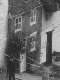
\includegraphics[width=0.8\textwidth]{escala/128_86_viz.png}
        \caption{~\texttt{vizinho}.}
    \end{subfigure}%
    \hspace{8pt}
    \begin{subfigure}{0.33\textwidth}
        \centering
        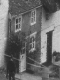
\includegraphics[width=0.8\textwidth]{escala/128_86_bil.png}
        \caption{~\texttt{bilinear}.}
    \end{subfigure}
    \\[8pt]
    \begin{subfigure}{0.33\textwidth}
        \centering
        \includegraphics[width=0.8\textwidth]{escala/128_86_bic.png}
        \caption{~\texttt{bicubica}.}
    \end{subfigure}%
    \hspace{8pt}%
    \begin{subfigure}{0.33\textwidth}
        \centering
        \includegraphics[width=0.8\textwidth]{escala/128_86_lag.png}
        \caption{~\texttt{lagrange}.}
    \end{subfigure}

    \caption{Redimensionamento para $80 \times 60$ aplicado em \texttt{city128.png} ($128 \times 128$).}
    \label{fig:esc:86}
\end{figure}